\documentclass[aspectratio=1210]{beamer}

\input{.setup.tex}

\title{Ausnutzung von Prozessorlücken} 
\author{Enrico Stemmer}

\begin{document}

\begin{frame}
	\titlepage
\end{frame}

\begin{frame}
	\frametitle{Übersicht}
	\tableofcontents
\end{frame}

\section{Einleitung}
\subsection{Vorstellung}
\begin{frame}{\insertsubsection}
	\begin{itemize}
		\item \textbf{Name:} Enrico Stemmer
		\item \textbf{Hobby:} Programmieren
		\item \textbf{Beruf:} Dualer student bei ARCA-Consult (Softwareentwickler)
		      \customnote{Beratung für IT Security und Informationssicherheit.}
		      \customnote{Warum THEMA: Vorher schon von Spectre gehört, spekulative Ausführung}
		      \vspace{0.5cm}
		\item Code + Präsentation auf \href{https://github.com/h3rmt-thi/seminar_4}{\texttt{https://github.com/h3rmt-thi/seminar\_4}}
		      \customnote{Fragen zwischendurch gerne stellen.}
	\end{itemize}
\end{frame}

\subsection{Einführung}
\begin{frame}{\insertsubsection\ (Was sind Prozessorlücken?)}
	\begin{itemize}
		\item \textbf{Ziel:} Arbeitsspeicher auslesen
		\item Speicherisolation durch Betriebssystem wird umgangen
		      \customnote{*OS* separiert Speicherbereiche, damit Programme <br>nicht aufeinander zugreifen können. MMU (Memory Management Unit)}
		      \customnote{In Prozessen mit `mprotect` oder V8 JavaScript Isolates}
		      \customnote{Ohne mehr rechte (sudo)}
		\item Zugriff auf fremden Speicher (Programme, Kernel, VMs)
		      \customnote{Cloudcomputing als angriffsziel, weil viele VMs auf einem Server}
		\item Es muss bereits Code auf dem Zielsystem ausgeführt werden
		      \customnote{aber auch JS auf webiste an sich code execution}
		      \customnote{gibt remote spectre}
	\end{itemize}
\end{frame}

\section{Grundlagen moderner CPU-Architekturen}
\subsection{Arbeitsspeicher}
\begin{frame}{\insertsection\\\insertsubsection}
	\begin{itemize}
		\item Hirarchie: Register, Cache (L1, L2, L3), RAM
		\item Datentransfer zwischen CPU und RAM langsam
		      \customnote{mehrere 100 Zyklen in der Zeit}
		\item Cache schneller, weit unter 100 Zyklen
	\end{itemize}
\end{frame}

\subsection{CPU}
\begin{frame}[fragile]{\insertsection\\\insertsubsection}
	\begin{itemize}
		\customnote<1>{Moderne Prozessoren so schnell weil Sachen im Voraus oder parallel gemacht werden.}
		\item<1-> \textbf{Out-of-Order Execution:} Ausführen von Befehlen in geänderter Reihenfolge
		\item<2-> \textbf{Speculative Execution:} Ausführen von vermuteten Befehlen
		\item<3-> \textbf{Branch Prediction:} Vorhersage von Verzweigungen
	\end{itemize}

	\begin{center}
		\begin{onlyenv}<1>
			\begin{minipage}{0.3\textwidth}
				\begin{block}{Code Example}
					\begin{minted}[breaklines]{c}
int a = 5;
int b = 10;

int c = a + b;
int d = c * 2;

int e = a - b;
int f = e / 2;
                    \end{minted}
				\end{block}
			\end{minipage}
		\end{onlyenv}

		\begin{onlyenv}<2>
			\begin{minipage}{0.4\textwidth}
				\begin{block}{Code Example}
					\begin{minted}{c}
int a = 5;
int b = 10;
int result = 2;

if (a + b > 20) {
    result = a * b;
}
                    \end{minted}
				\end{block}
			\end{minipage}
		\end{onlyenv}

		\begin{onlyenv}<3>
			\begin{minipage}{0.6\textwidth}
				\begin{block}{Code Example}
					\begin{minted}{c}
int u = 0;
for (int i = 0; i < 10; i++) {
    if (i < 9) {
        u += i * 5;
    }
}
                    \end{minted}
				\end{block}
			\end{minipage}
		\end{onlyenv}
	\end{center}
\end{frame}

\section{Spectre}
\begin{frame}[fragile]{\insertsection}
	\begin{tikzpicture}[remember picture,overlay]
		\node[anchor=north east, xshift=-0.2cm, yshift=-0.2cm] at (current page.north east) {
			
\includegraphics[width=1.5cm]{spectre_small.png}
		};
	\end{tikzpicture}

	\begin{itemize}
		\item \textbf{Side Channel:} nutzen indirekter Informationen
		      \customnote<1>{Stromverbrauch, Zeit, Ton?}
		\item Cache als Sidechannel, Speculative Ausführung als Angriff
		      \customnote<1>{Genau: spec execution führt code aus der daten in cache lädt}
		\item Zeitmessung des Datenzugriffs als Indikator
	\end{itemize}

	\begin{onlyenv}<2>
		\begin{itemize}
			\item \textbf{1. Juni 2017:} Hardwarehersteller informiert
			      \customnote<2>{Betrifft alle modernen CPUs mit spekulativer Ausführung.}
			\item \textbf{3. Januar 2018:} Spectre und Meltdown veröffentlicht
			      \customnote<2>{JETZT code beispiel + fragen}
		\end{itemize}
	\end{onlyenv}

	\begin{onlyenv}<3>
		\begin{itemize}
			\item \textbf{Spectre v2:} Variante nutzt indirekte Sprungvorhersage
			      \begin{itemize}
				      \item Moderne CPUs nutzen Branch Prediction Unit (BPU)
				      \item Training der BPU mit kontrollierten Sprungzielen
				      \item Spekulative Ausführung nutzt manipuliertes Sprungziel
				      \item Leak sensibler Daten über Side Channels
				            \customnote<3>{Unterschied: BPU geshared -> code in anderem context kann auf manipulierter Funcktion des angreifers landen}
			      \end{itemize}
		\end{itemize}
	\end{onlyenv}

	\begin{onlyenv}<4-5>
		\begin{itemize}
			\item \textbf{Gegenmaßnahmen:}
			      \begin{itemize}
				      \begin{onlyenv}<4-5>
					      \item Linux: \textit{lfence}, \textit{nospec}
					      \customnote<4>{lfence: Warten bis alle vorherigen mem loads abgeschlossen sind => CPU bricht Spec Exec ab}
					      \customnote<4>{nospec: Abbrechen von Spec Exec wenn array access out of bounds}
					      \item Firefox, Webkit: Timing Genauichkeit reduziert
					      \customnote<4>{Damit Cache Timing nicht mehr möglich ist}
					      \item Chrome: Sandboxing
					      \customnote<4>{Eingenen prozess pro Tab}
					      \customnote<4>{+JIT maskiert pointer auf JS arrays und Strings}
				      \end{onlyenv}
				      \begin{onlyenv}<5>
					      \item IBRS (Indirection Branch Restricted Speculation)
					      \customnote<5>{Hardware fixes}
					      \customnote<5>{Braucht Microcode Suport, kernel aktiviert es}
					      \customnote<5>{Verhindert Spekulation in indirekten Sprüngen}
					      \customnote<5>{https://lwn.net/Articles/743019/}
					      \item STIBP (Single Thread Indirect Branch Predictors)
					      \customnote<5>{Kein Sharing der BPU zwischen Threads}
					      \customnote<5>{https://shorturl.at/MkOs6}
					      \item IBPB (Indirect Branch Prediction Barrier)
					      \customnote<5>{Verhindet Manipulieren von BPU über Ring switches}
				      \end{onlyenv}
			      \end{itemize}
		\end{itemize}
	\end{onlyenv}
\end{frame}

\section{Meltdown}
\begin{frame}[fragile]{\insertsection}
	\begin{tikzpicture}[remember picture,overlay]
		\node[anchor=north east, xshift=-0.2cm, yshift=-0.2cm] at (current page.north east) {
			
\includegraphics[width=1.5cm]{meltdown_small.png}
		};
	\end{tikzpicture}
	\begin{itemize}
		\item<1-> Betrifft nur Intel x86, nicht AMD
		      \customnote<1>{Auch manche ARM und IBM PowerPC}
		\item<1-> \textbf{Ziel:} Kernel-Speicher auslesen
		\item<2-> Out-of-Order Execution führt Check und Laden gleichzeitig aus (Lesen wartet nicht auf Berechtigungscheck)
		      \customnote<2>{Erst nachemd check wird rollback oder commit gemacht}
		\item<2-> Abfangen der SigSegV durch \texttt{segfault\_handler}
		      \customnote<2>{SigSegV: Segmentation Fault, Zugriff auf nicht erlaubten Speicher}
		      \customnote<2>{JETZT code beispiel + fragen}
		\item<3-> \textbf{Gegenmaßnahmen:}
		      \begin{itemize}
			      \item KPTI (Kernel Page Table Isolation)
			            \customnote<3>{Kernel und User-Speicher in verschiedene Page Tables (nicht mehr gemapped)}
			            \customnote<3>{Vorher in einen NS gemapped, und durch checks gesichert}
			      \item Hardware Fixes
		      \end{itemize}
	\end{itemize}
\end{frame}

\section{Rowhammer}
\begin{frame}{\insertsection}
	\begin{itemize}
		\customnote<1>{June 2014 an DDR3 RAM entdeckt}
		\customnote<1>{Rowhammer ist ein Hardwarefehler, der durch wiederholtes Zugreifen auf benachbarte Speicherzellen in DRAM-Modulen verursacht wird.}
		\item<1-> \textbf{Ziel:} Modifizieren von Speicherzellen
		\item<1-> Wiedeholtes Zugreifen auf benachbarte Speicherzellen
	\end{itemize}

	\begin{onlyenv}<2->
		\begin{itemize}
			\item Erzeugen von Bitflips in benachbarten Zellen durch kompkate Architektur von DRAM.
			      \customnote<2>{Rowhammer.js: JavaScript-Implementierung}
			      \customnote<2>{Double-Sided Rowhammer}
			      \customnote<2>{Half-Double: weiter entfernten Zeilenle: weiter entfernten Zeilen}
			\item \textbf{Gegenmaßnahmen:}
			      \begin{itemize}
				      \item EEC (Error-Correcting Code)
				            \customnote<2->{Detektion und Correction, normal manachmal Detection}
				            \customnote<2->{Ein extra Bit pro Byte}
				      \item TRR (Target Row Refresh)
				            \customnote<2->{Automatisches Refreshen von benachbarten Zeilen bei häufigem Zugriff}
				            \customnote<2->{Optional im DDR4 Standard, propietär}
			      \end{itemize}
		\end{itemize}
	\end{onlyenv}

	\begin{center}
		\begin{onlyenv}<1>
			\vspace{0.5cm}
			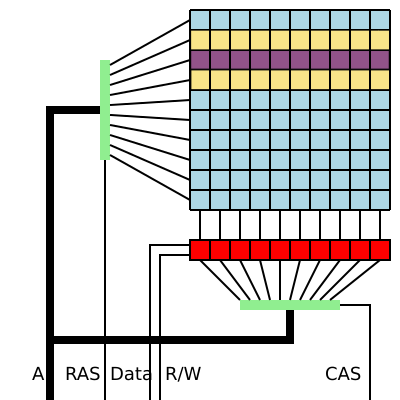
\includegraphics[width=5cm]{rowhammer.png}
			\vspace{0.5cm}
		\end{onlyenv}
	\end{center}
\end{frame}


\end{document}